% Réflexions sur quels blocs utiliser pour détecter ce signal

Vous savez maintenant comment transformer l'onde sonore du claquement de doigts en un signal électrique que vous pouvez filtrer et observer au microscope. Lors des prochains hands-on (la semaine prochaine), vous implémenterez le circuit qui permet de détecter automatiquement ce claquement. Selon vous, comment feriez-vous pour détecter ce signal, de manière générale sans penser encore à l'implémentation à l'aide de composants électroniques? Quelles "fonctions" électroniques utiliseriez-vous pour passer du signal observer aujourd'hui à un signal de commande tel qu'illustré ci-dessous?

\begin{figure}[!ht]
	\centering
	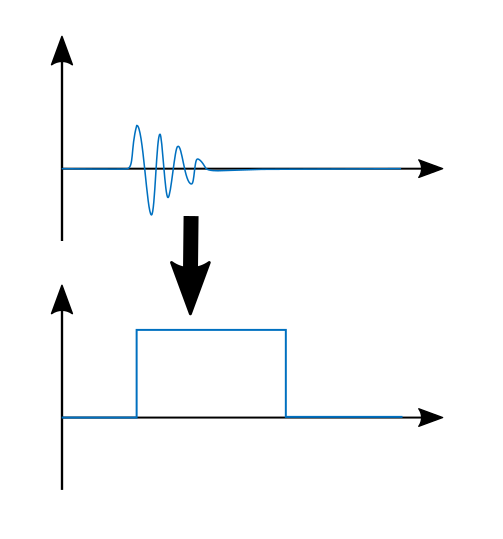
\includegraphics[width=.6\textwidth]{figures/signals.PNG}
	\caption{Détection d'un claquement de doigts}
	\label{fig:signals}
\end{figure}